\begin{frame}{Named Entity Disambiguation : Outline}
 \begin{itemize}
  \item Techniques
  \begin{itemize}
   \item Local Disambiguation \medskip
   \item Collective Disambiguation \medskip
   \item Robust Disambiguation of Named Entities \medskip
  \end{itemize}
  \item Quick Demo
 \end{itemize}

\end{frame}
\begin{frame}{Local Disambiguation}
 \begin{itemize}
  \item Resolve each mention oblivious to the other disambiguations \medskip
  \item Need to disambiguate a mention by collecting the local evidences \medskip
  \item \textbf{Evidences}  POS tags, gender information, dictionary lookup \medskip
  \item \textbf{Local}  We cannot use the disambiguation information for any of the other entities for solving the problem \medskip
  \item Techniques
  \begin{itemize} 
  \item Machine Learning Based
  \item Rule Based
  \item Recent Rule based 
 \end{itemize}
 \end{itemize}
 

\end{frame}
\begin{frame}{Local Disambiguation : Rule Based}
\begin{itemize}
 \item Stems from the classical problem of word sense disambiguation \medskip
 \item Example : Lesk's Algorithm \medskip
  \begin{block}{Lesk's Algorithm} \medskip
       
 For each mention, pick the candidate sense for which there is maximum overlap
 in the gloss (definition) of the candidate and the context
\end{block}
\item Note that the possible mentions are those that are identified by the named entity recognizer
 \end{itemize}

 
\end{frame}


\begin{frame}{Local Disambiguation : Rule Based (Example)}
\begin{itemize}
\item Consider the same example
 \begin{figure}[h]
 \centering
 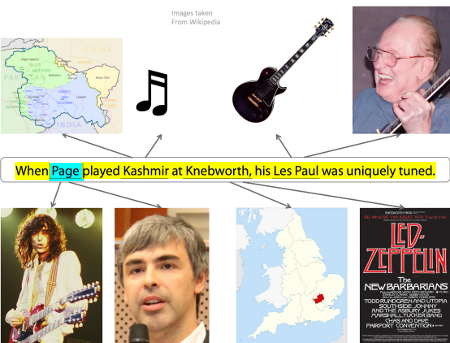
\includegraphics[bb=0 0 216 165]{./nedrulebased.png}
 % ned.png: 450x343 pixel, 150dpi, 7.62x5.81 cm, bb=0 0 216 165
 \caption{Disambiguating ``Page``}
\end{figure}
\item Disambiguating ``Page''
\end{itemize}
\end{frame}
\begin{frame}{Local Disambiguation : Rule Based (Example)}
 \begin{itemize}
  \item \textbf{Jimmy Page}\footnote{First para of the Wikipedia Entry} James Patrick "Jimmy" Page, OBE (born 9 January 1944) is an English musician, songwriter and record producer who achieved international success as the \textcolor{red}{guitar player} and leader of the rock band Led Zeppelin.
  \item \textbf{Larry Page}\footnote{First para of the Wikipedia Entry}	 Lawrence "Larry" Page[2] (born March 26, 1973) is an American Business magnate and computer scientist who is the co-founder of Google, alongside Sergey Brin. On April 4, 2011, Page succeeded Eric Schmidt as the chief executive officer of Google.[3][4] As of 2014, Page's personal wealth is estimated to be US\$32.3 billion, ranking him \#19 on the Forbes list of billionaires.[1]
  \item \textbf{Context} \textcolor{red}{played} kashmir at Knebworth, his Les paul was uniquely tuned
  
 \end{itemize}
\textcolor{green}{\textbf{\emph{Pick the candidate that is most likely given the context}}}
\end{frame}
\begin{frame}{Local Disambiguation : Rule based : Drawbacks}
\begin{itemize}
 \item Context can be misleading \bigskip
 \textcolor{green}{\emph{Amazon} saw a flood of visitors} \bigskip
 \item Context can be insufficient (or even absent!) \bigskip
 \item Rule based disambiguation has made a comeback with AIDA \bigskip
 \item ML based local disambiguation to come
 
 
\end{itemize}

 
\end{frame}